\documentclass[11pt]{article}
\RequirePackage{cmap}%
\usepackage[a4paper, hmargin={2.8cm, 2.8cm}, vmargin={2.5cm, 2.5cm}]{geometry}
\usepackage{eso-pic} % \AddToShipoutPicture
\usepackage{graphicx} % \includegraphicsud over
\usepackage[utf8]{inputenc} % æøå
\usepackage[T1]{fontenc} % mere æøå
\usepackage{verbatim} % så man kan skrive ren tekst
\usepackage{listings} % kode
\usepackage[round, sort, numbers]{natbib} %citationer i chicago format
\usepackage{amsmath} % flere matematikkommandoer
\usepackage[british,UKenglish,USenglish,english,american]{babel} % orddeling
\usepackage[all]{xy} % den sidste (avancerede) formel i dokumentet
\usepackage{graphicx} %for billedhåndtering
\usepackage{listings} %algoritmer og programming language
\usepackage{diagbox}
\usepackage[titletoc,title]{appendix}
\newcommand{\listappendicesname}{Appendices}
\lstset{
basicstyle=\ttfamily\small,
columns=fullflexible,
language=Python,
tabsize=2,
numbers=left,
showstringspaces=false,
}

\usepackage{fancyhdr} %header, footer
\usepackage{hyperref}
\usepackage{multirow}
\usepackage{pdfpages}
\usepackage{multicol}
\usepackage{fancyhdr}
\usepackage{clrscode3e}
\usepackage{indentfirst}
\usepackage{wrapfig}
\usepackage{units}
\newcommand{\citat}[2]{\begin{justify}\textit{``#1''}\hspace{0.1cm}\footnote{#2}\end{justify}}
\author{
 \textsc{\Large{Amr El Sayed}}\\
 \textsc{\Large{KuId - vwj159}}}
 \title{
  \vspace{3cm}
  \textsc{\Huge{Project Outside the Course Scope}}\\
  \vspace{0.5cm}
  \textsc{\Large{Closure Plots for Basic Arithmetics}}\\
  %\vspace{11.5cm}
}
\lstdefinelanguage{JavaScript}{
  keywords={typeof, new, true, false, catch, function, return, null, catch, switch, var, if, in, while, do, else, case, break},
  keywordstyle=\color{blue}\bfseries,
  ndkeywords={class, export, boolean, throw, implements, import, this},
  ndkeywordstyle=\color{darkgray}\bfseries,
  identifierstyle=\color{black},
  sensitive=false,
  comment=[l]{//},
  morecomment=[s]{/*}{*/},
  commentstyle=\color{purple}\ttfamily,
  stringstyle=\color{red}\ttfamily,
  morestring=[b]',
  morestring=[b]"
}

\begin{document}

%% Change `ku-farve` to `nat-farve` to use SCIENCE's old colors or
%% `natbio-farve` to use SCIENCE's new colors and logo.
\AddToShipoutPicture*{\put(0,0){\includegraphics*[viewport=0 0 700 600]{ku-farve}}}
\AddToShipoutPicture*{\put(0,602){\includegraphics*[viewport=0 600 700 1600]{ku-farve}}}

%% Change `ku-en` to `nat-en` to use the `Faculty of Science` header
\AddToShipoutPicture*{\put(0,0){\includegraphics*{kuen1}}}

\clearpage\maketitle
\thispagestyle{empty}
\newpage
\begin{center}{\huge\textbf{Closure Plots for Basic Arithmetics}}\newline \textit{\\DIKU - Project Outside the Course Scope}\end{center}
\hfill \break
\begin{tabular}{l l l }
\textbf{Students Names} &: &Amr El Sayed - VWJ159\\\\
\textbf{University} &:& University of Copenhagen\\\\
\textbf{Institution} &:& Department of Computer Science (DIKU)\\\\
\textbf{General Supervisor} &:& Michael Kirkedal Thmosen\\\\
\textbf{Practical Supervisor} &:& Oleksandr Shturmov\\\\
\textbf{Period} &:& Block 5\\\\
\textbf{Year} &:& 2016\\\\
\textbf{Pages} &:& \\\\
\textbf{Github} &:& \url{https://github.com/Amr116/ClosurePlots}\\
\end{tabular}
\\\\\\\\\\\\\\
\begin{center}{\huge\textbf{Certificate}}\end{center}

This is to certify that the work contained in the thesis entitled "Closure Plots for Basic Arithmetics" by Amr El Sayed has been carried out under our supervision and that this work has not been submitted elsewhere.\\\\\\\\
\begin{center}\noindent\rule{8cm}{0.4pt}%\end{center}

\begin{tabular}{ l l l c r l l l}\\
    %~\ ~\ ~\ ~\   %~\ ~\ 
    \textbf{General Supervisor} & & & & & & \textbf{Practical Supervisor} \\
    Michael Kirkedal Thmosen & & & & & & Oleksandr Shturmov\\
    m.kirkedal@di.ku.dk & & & & & & oleks@di.ku.dk\\
    Department of Computer Science (DIKU) & & & & & & Department of Computer Science (DIKU)\\
    University of Copenhagen & & & & & & University of Copenhagen\\
\end{tabular}
%\begin{center}
%\textbf{Supervisor}\\
%Michael Kirkedal Thmosen \\
%m.kirkedal@di.ku.dk \\
%Department of Computer Science DIKU \\
%University of Copenhagen
%\end{center}
\end{center}
\newpage
\section{Abstract}
%%%%%%%%%%%%%%%%%%%%%%%%%%%%%%%%%%%%%%%%%%%%%%%%%%%%%%%%%%%%%%%%%%%%%%%%%%%%%%%%%%%%%%%%%%%%%%%%%%%%%%%%%%%%%%%%%%%%%%
%As computer systems continue to grow rapidly in both complexity and scale, developers need tools to help them understand the behavior and performance of these systems.  While information visualization is a promising technique, most existing computer systems visualizations have focused on very specific problems and data sources, limiting their applicability.
%%%%%%%%%%%%%%%%%%%%%%%%%%%%%%%%%%%%%%%%%%%%%%%%%%%%%%%%%%%%%%%%%%%%%%%%%%%%%%%%%%%%%%%%%%%%%%%%%%%%%%%%%%%%%%%%%%%%%%
%However, simulations with rounded arithmetic are simply guesses and guidance, not proof of anything.\\
%The floating point has computation lacks mathematical rigor, and the simulations with rounded arithmetic are simply guesses and guidance, not proof of anything, and since a rounded number is by definition the substitution of an incorrect number for the correct one. Therefore The purpose of " Closure Plots for Basic Arithmetics"  is to create visualization tool for illustrate basic arithmetics simulation to floating point during, and then highlight the bits lacks to those elementary operations.\\
\section*{Resume}

\newpage
\begin{center}
\tableofcontents
\end{center}

\newpage
\section{Introduction}
I am a third year computer science student at the University of Copenhagen, I'm enrolled in the undergraduate (bachelor) part of the education. This report is the final product of a 1-block Project Outside the Course Scope. This paper covers the development process of Closure Plots for Basic Arithmetics on those aspects of floating-point that have a direct impact on designers of computer systems.

\subsection{Purpose}
The purpose of this document is divided into two purposes:\\

The first purpose is to describe the UI to Closure Plots for Basic Arithmetics application for instructors and Computer Science students at Department of Computer Science - University of Copenhagen, so they can easily interact with the application.\\

The second purpose is explain the requirement specifications for Closure Plots for Basic Arithmetics application and explain the steps of implement this project to help the developers to further developing this application.


%The purpose of this document is to describe the requirement specifications for Closure Plots for Basic Arithmetics application for instructors and Computer Science students at Department of Computer Science - University of Copenhagen, and to explain the steps of implement and design this project to help the developers to further developing this application.

%help the developers to further developing the application, and also it will help instructors and Computer Science students at Department of Computer Science - University of Copenhagen to understand the application and how to interact with e.g. by adding some variables in the mathematical operations or understand the data presented in the application. %Closure Plots

\subsection{Intended Audience and Reading Suggestions}
This document is intended for readers who have studied Computer Science or similar, or are simply interested in the field of IT. Readers are assumed to have basic programming knowledge and some familiarity with web development technologies.

\subsection{Project Scope}
The software to be produced is a Closure Plots for Basic Arithmetics, which will be referred to as "CPBA" thorough this document.\\

CPBA will allow students to learn about the behaviour of basic arithmetic operations in floating point arithmetic with different precision through interaction with UI. The CPBA will also allow the instructors and creative students to modify the variables in arithmetic operations to monitor behaviour of floating point.\\

The objective of CPBA application is to be visualization tool for illustrating the behaviour of basic arithmetic operations (e.g., Addition, Subtraction, Multiplication, Division) in floating point arithmetic with different precision (e.g., Half, Single, Double, Quadruple).\\



%This paper covers the development process of Closure Plots for Basic Arithmetics on those aspects of floating-point that have a direct impact on designers of computer systems, and is intended for readers who have studied Computer Science or similar, or are simply interested in the field of IT. Readers are assumed to have basic programming knowledge and some familiarity with web development.\\

%The purpose of this project is to create a visualization tool for illustrating the behaviour of basic arithmetic operations (e.g., Addition, Subtraction, Multiplication, Division) in floating point arithmetic with different precision (e.g., Half, Single, Double, Quadruple).\\

\section{Overall Description}%عموما الوصف
Floating-point arithmetic is considered an esoteric subject by many people. This is rather surprising because floating-point is ubiquitous in computer systems. Almost every language has a floating-point datatype, computers from PCs to supercomputers have floating-point accelerators, most compilers will be called upon to compile floating-point algorithms from time to time, and virtually every operating system must respond to floating-point exceptions such as Overflow, Undeflow, Infinity and Inexpressible.\\

In computing\footnote{Computing is any goal-oriented activity requiring, benefiting from, or creating a mathematical sequence of steps known as an algorithm — e.g. through computers. Computing includes designing, developing and building hardware and software systems, processing, structuring, and managing various kinds of information, doing scientific research on and with computers, making computer systems behave intelligently, and creating and using communications and entertainment media.}, floating point is the formulaic representation that approximates a \textbf{real number}, that include all the rational numbers, such as the integer -5 and the fraction 4/3, and all the irrational numbers, such as $\sqrt{2}$ (1.41421356…, the square root of 2, an irrational algebraic number). Included within the irrationals are the transcendental numbers, such as $\pi$ (3.14159265…), so as to support a trade-off between range and precision. A number is, in general, represented approximately to a fixed number of significant digits (the significand) and scaled using an exponent in some fixed base.\\

The most popular code for representing real numbers is called the IEEE Floating-Point Standard, that have three basic components: the sign, the exponent, and the mantissa. The mantissa is composed of the fraction and an implicit leading digit. The exponent base (2) is implicit and need not be stored.\\
%\textit{The sign} bit is as simple as it gets. 0 denotes a positive number, and 1 denotes a negative number. Flipping the value of this bit flips the sign of the number.\\
%\textit{The exponent} field needs to represent both positive and negative exponents. To do this, a bias is added to the actual exponent in order to get the stored exponent. For single-precision floats, this value is 127. Thus, an exponent of zero means that 127 is stored in the exponent field. A stored value of 200 indicates an exponent of (200-127), or 73. For reasons discussed later, exponents of -127 (all 0s) and +128 (all 1s) are reserved for special numbers. For double precision, the exponent field is 11 bits, and has a bias of 1023.

%the base for the scaling is normally two, ten, or sixteen. A number that can be represented exactly is of the following form:\\

%This project is based on the principle of float in the floating point, which is derived from the fact that there is no fixed number of digits before and after the decimal point; that is, the decimal point can float, therefore the implementing of this project focuses on create a visualization tool for illustrating the behaviour of basic arithmetic operations (Addition, Subtraction, Multiplication, Division) to integer number with different precision (Half, Single, Double, Quadruple), and also create the infrastructure that will allow for future development to representing different code for floating point eg. IEEE Floating-Point Standard or something else on this approach.

%There are also representations in which the number of digits before and after the decimal point is set, called fixed-pointrepresentations.\\

%This report is divided into four parts ( Analysis, Design ,Implementation and Testing ).\\
%For the analysis part, I will discuss the requirements that are needed to implement the project and compare to some of the technology, which can achieve the goals of this project, and to show the strengths and weaknesses of this technology.\\\\
%For the design part, I will introduce tools and techniques that have been chosen to implement the project and to clarify whether it is possible to achieve all the objectives of this project through the chosen technologies.\\\\
%For the implementation part, I will explain the method of execution to achieve the specification of this project based on the design part, and i will explain each function and method separately.\\\\
%For the test part, I will an investigation conducted to provide with information about the quality of the product ( application ) with the intent of finding bugs (errors or other defects), and It would achieve the benefit of the development in the future.\\

\subsection{Product Perspective}% وجهة نظر المنتج
A simple way to illustrating the behaviour of basic arithmetic operations, that is by someone sitting physically at a computer or with paper and write down the numbers and finish this calculation process. There are tools available, commercial or open source that support arithmetic operations to digits or binary numbers. Many Operating Systems and applications themselves come with calculator support those basic arithmetic operations. But unfortunately, all these tools usually require a person sitting physically at a computer writing down the numbers one by one.\\

Thus the need for a web based application to be a visualization tool for illustrating the behaviour of basic arithmetic operations.

\subsection{Product Features}% مواصفات المنتج
The software is used mainly to illustrating the behaviour of basic arithmetic operations in floating point arithmetic with different precision of web based software so the user who is maintaining can access it from virtually any where.\\

This software is based on the principle of float in the floating point, which is derived from the fact that there is no fixed number of digits before and after the decimal point; that is, the decimal point can float, therefore the implementing of this project focuses on create a visualization tool for illustrating the behaviour of basic arithmetic operations (Addition, Subtraction, Multiplication, Division) to integer number with different precision (Half, Single, Double, Quadruple), and also create the infrastructure that will allow for future development to representing different code for floating point eg. IEEE Floating-Point Standard or something else on this approach.

\section{Analysis}
In this section we will be analysing the problem described above. The analysis will be focused on narrowing in special areas of the problem domain that will be central to designing and implementing a working prototype.
\subsection{Different precision}% to represent a number
%One obvious weakness when designing the application that is different precision to floating point. As human, we can represent those different precisions by their arithmetic definition.
Different precision in floating point is one of the obvious shortcomings when designing the application, if we could not represent those precision with their actual digit length.\\
We can see the mathematical notation to those precisions as:
%Manual representation by human can represent those precisions as:
\begin{itemize}
\item{Half-precision is $2^{16}$}
\begin{itemize}\item[]{The positive numbers for this precision is range between 0 to 65535.}\end{itemize}
\item{Single-precision is $2^{32}$}
\begin{itemize}\item[]{The positive numbers for this precision is range between 0 to 4294967295.}\end{itemize}
\item{Double-precision is $2^{64}$}
\begin{itemize}\item[]{The positive numbers for this precision is range between 0 to 18446744073709551615.}\end{itemize}
\item{Quadruple-precision is $2^{128}$}
\begin{itemize}\item[]{The positive numbers for this precision is range between 0 to \\340282366920938463374607431768211455.}\end{itemize}
\end{itemize}

But, does programming languages represent those precisions such as the way in which it represented in mathematical notation?\\
Some programming languages have maximum length of digit with different precisions, and if those digits has overflow the maximum length, then it representing in scientific notation or in rounding format\footnote{Rounding means making a number simpler but keeping its value close to what it was. }. This scientific notation will require redefining the length of those digit to be able to participation in arithmetic operations, otherwise we will get wrong results.\\\\
The below table\ref{max}  showing represent digit length for different precisions to different languages. From this table we can see the similarities and differences in the representation of length for different precisions. This difference will be among the main reasons for choosing the design and implementation of this project.\\
\begin{table}[h]
\centering
\small
\label{max}
\begin{tabular}{|c|c|c|c|}
\hline
\multirow{2}{*}{\diagbox[width=5em]{DP}{PL}}
          & \multirow{2}{*}{JavaScript} & \multirow{2}{*}{Python}                 &\multirow{2}{*} {GO} \\ 
          &                             &                                         &   \\ \hline
Half      & 65536                       & 65536                                   &  65536\\ \hline
Single    & 4294967296                  & 4294967296                              &  4.294967296e+09 \\ \hline
Double    & 18446744073709552000        & 18446744073709551616                    &  1.8446744073709552e+19 \\ \hline
Quadruple & 3.402823669209385e+38       & 340282366920938463463374607431768211456 &  3.402823669209385e+38  \\ \hline
\end{tabular}
\caption{Representation of maximum digit length with different precisions at some programming language}
\end{table}\\
%Some of programming langauges have maximum length to represent digits with different precisions, until it gets to represent those numbers in scientific notation, and I will not be happy for that, because it will required some extra work to represent big numbers, and to do some arithmetic operation with scientific notation numbers.\\
%fx. If we will take JavaScript as primary programming language to CPBA project, then we can see what is the maximum length to represent Double and Quadruple precisions, which are scientific notation numbers.

\subsection{Viewport Size vs bit Pixel}% to represent a number
The browser viewport is the size of the rectangle that a web page fills on your screen. It’s basically the size of the browser window, less the toolbars and scrollbars. It’s the bit of the screen we are actually using to show the webpage.\\
%But, how is possible the visualization tool for illustrating the behaviour of basic arithmetic operations can show all those elements in the screen.
Is it possible the CPBA application to illustrating the behaviour of basic arithmetic operations in the viewport size !?\\
%We want to calculate arithmetic operations (e.g. Addition, Subtraction, Multiplication, Division) to integer number with different precision (Half, Single, Double, Quadruple), and to do those calculations we need at least need two variables, that is mean if variable X and Y have Single precision, then we will need to represent the result of arithmetic operations  to X and Y, which will give us $65536^{2} = 4294967296$ element, that need to be apparent to user in the Viewport.
We want to calculate arithmetic operations (e.g. Addition, Subtraction, Multiplication, Division) to integer number with different precision (Half, Single, Double, Quadruple), and to do those calculations we need at least two variables, that is mean if variables X and Y have Single precision, so we will need to represent the result of this arithmetic operations, which will give us $65536^{2} = 4294967296$ elements.\\\\
This huge number of elements can not be shown in the Viewport while maintaining achieve a clear vision for each element separately. So we need some way to allow us to achieve a clear vision for each element and also allows the user to take advantage of this visualization tool for illustrating the behaviour of basic arithmetic operations.\\
\section{Design}
To make this application easily accessible for the students, I decided that it should be web-based: meaning that it should be accessed via internet by using a standard web browser or students can get to the project files from  a physical source (e.g. flash memory). This way there would be no need to distribute the program and all of the required packages for it to run, which we would need if i had to make a program that was not web-based. By making the application web-based, I ensure the accessibility of it for most, if not all, users.
The solution will not target mobile/tablet users specifically.\\

Since this project should be web-based application, so i need to use HTML and CSS, because they are two of the core technologies for building Web pages, but to build the functionality of this project i can choose between many programming languages, but only JavaScript is the only ones that fit the CPBA requirement, because users can get access to CPBA via internet or offline if they get the project like physical source.\\\\
%To make this application easily accessible for the students, I decided that it should be web-based: meaning that it should be accessed via internet by using a standard web browser. This way there would be no need to distribute the program and all of the required packages for it to run, which we would need if we had to make a program that was not web-based. By making the application web-based, I ensure the accessibility of it for most, if not all, users. The solution will not target mobile/tablet users specifically, but they should be able to use the website nonetheless.
%%%%%%%%%%%%%%%%%%%%%%%%%%%%%%%%%%%%%%%%%%%%%%%%%%%%%%%%%%%%%%%%%%%%%%%%%%%%%%%%%%%%%%%%%%%%%%%%%%%%%%%%%%%%%%%%%%%%%%%%%%%%%%%
%Since i decided on a web-based application i needed a server, and this presented some challenges of it's own.
The above section (Analysis) I’ve discussed some of the problems that will confront us in the design and implementation of this project, therefore in the below subsection, i will re-presentation of these problems and explain my ideas for the design and implementation of the solution to these problems.\\
\subsection{Arithmetic operations \& Different precision}
The user need a simple way to illustrating the behaviour of basic arithmetic operations (Addition, Subtraction, Multiplication, Division) with different precision (Half, Single, Double, Quadruple), therefore the project should give the possibility for user to select and choice between different arithmetic operations and different precision. For this reason, i decided the front-end design of CPBA should include  two  <select> tags, which create a drop-down list, and thereby I collect user input from the selected option.
\subsection{Mathematical notation}
where have been chosen javascript as primary programming language to the functionality of this project, because it will provide access possibility of user via online or offline, but does Javascript represent precisions such as the way in which it represent in mathematical notation. Unfortunately, The answer is No, because the maximum integer can be represent of JavaScript is $2^{31} -1$, or $2147483647$, otherwise the integer will be represent in scientific notation. That's why I decided to make CPBA is limited to precisions Half and Single only.
\subsection{Elements}
To represent precisions Half and Single, that will give huge number of elements, which need to be shown in viewport, but to represent all those elements at once will not give the possibility to users to see and illustrating the behaviour of basic arithmetic operations, therefore in CPBA I need to summarize the those elements to miniature form.\\
This form differs from precision to other precision in the number of stages. In other words for example in addition operation for precision Half, we have $2^{16}$ element for variable X and $2^{16}$ for variable Y, so the sum of those two variables is $2^{32}$ elements.\\
I decide to show 256 elements of this result at each stage, where each element represents 4 edges from the real results as shows in figure \ref{edges}.\\
\begin{figure}[h]
    \centering
    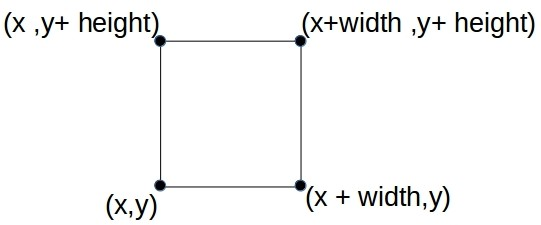
\includegraphics[width=0.5\textwidth]{edges}
    \caption{summarize form shows how each element represents in CPBA}
    \label{edges}
\end{figure}\\
The Half-precision will have four stages. At the first stage width and height will be equal to 4095, at the second stage will be equal to 255, at the third stage will be equal to 15,  and at the fourth (last stage) will be be equal to 0.\\\\
The Single-precision will have eight stages. At the first stage width and height will be equal to 268435455, at the second stage will be equal to 16777215, at the third stage will be equal to 1048575, at the fourth stage will be be equal to 65535, at the fifth stage will be be equal to 4095, at the sixth stage will be be equal to 255, at the seventh stage will be be equal to 15, and at the eighth stage (the last) will be be equal to 0\\\\
The below examples is Illustrative examples to prove of concept in addition operation of half precision at first stage form:\\\\
X = 4096, Y=53248\\
\scalebox{0.9}{
\begin{tabular}{lllll}
Leftmost bottom: &  4096  + 53248  &= 57344                  & ,57344  is less then $2^{16}$    & Correct\\
Rightmost bottom:& (4096 + 4095)  + 53248 &= 61439           & ,61439  is less then $2^{16}$    & Correct\\
Leftmost upper:  & 4096   + (53248 + 4095) &= 61439          & ,61439  is less then $2^{16}$    & Correct \\
Rightmost upper: & (4096  + 4095)  + (53248 + 4095) &= 65534 & ,65534  is less then $2^{16}$    & Correct\\
\end{tabular}
}\\\\
There are 4 correct and 0 Overflow, therefor i will show single Correct element represent this above range.\\\\
X = 4096, Y=57344\\
\scalebox{0.9}{
\begin{tabular}{lllll}
Leftmost bottom: &  4096  + 57344  & = 61440                  & ,61440  is less then $2^{16}$    & Correct\\
Rightmost bottom:& (4096 + 4095)  + 57344 & = 65535           & ,65535  is less then $2^{16}$    & Correct\\
Leftmost upper:  & 4096   + (57344 + 4095) & = 65535          & ,65535  is less then $2^{16}$    & Correct \\
Rightmost upper: & (4096  + 4095)  + (57344 + 4095) & = 69630 & ,69630  is more then $2^{16}$    & Overflow\\
\end{tabular}
}\\\\
There are 3 correct and 1 Overflow, therefor i will show single Mix element represent this above range.\\\\
%65536 65536
X = 4096, Y=61440\\
\scalebox{0.9}{
\begin{tabular}{lllll}
Leftmost bottom: &  4096  + 61440  & = 65536                  & ,65536  is more then $2^{16}$    & Overflow\\
Rightmost bottom:& (4096 + 4095)  + 61440 & = 69631           & ,69631  is more then $2^{16}$    & Overflow\\
Leftmost upper:  & 4096   + (61440 + 4095) & = 69631          & ,69631  is more then $2^{16}$    & Overflow \\
Rightmost upper: & (4096  + 4095)  + (61440 + 4095) & = 73726 & ,73726  is more then $2^{16}$    & Overflow\\
\end{tabular}
}\\\\
There are 0 correct and 4 Overflow, therefor i will show single Overflow element represent this above range.  
%%%%%%%%%%%%%%%%%%%%%%%%%%%%%%%%%%%%%%%%%%%%%%%%%%%%%%%%%%%%%%%%%%%%%%%%%%%%%%%%%%%%%%%%%%%%%%%%%%%%%%%%%%%%%%%%%%%%%%%%%%%%%

%Leftmost bottom:  1+1 = 2, 2 is less then $2^{16}$ result of correct\\
%Rightmost bottom: (1+4095)+1 = 4097, 4097 is less then $2^{16}$ result of correct\\
%Leftmost upper\enskip\enskip\enskip:   1+(1+4095) = 4097, 4097 is less then $2^{16}$ result of correct\\
%Rightmost upper\enskip\enskip:  (1+4095)+(1+4095) = 8194, 8194 is less then $2^{16}$ result of correct\\

\subsection{Forward, Back \& Reset}
While there will be many stages whether for Half precision and Single precision, therefore the users need for possibility to have mobile option, that can let the users move forward to next stage, back to previous stage or jump backward to first stage (Reset).\\\\
To move forward to next stage will be done when the user will click on the element, thereafter the element that it was clicked will be the first element of the next stage, and so on until width and height equal to zero, and hereby user has reached to the final stage.\\\\
To move back to previous stage will be done by click on back button, that button will provide the possibility to go back to previous stage until width and height equal to value 4095 in Half-precision or value 268435455 in Single-precision.\\\\
To reset or to jump back to first stage will be done by click on reset button, that button will assign width and height to 4095 in Half-precision or 268435455 in Single-precision.
%\subsection{What?}
%What we need basic arithmetic operations (e.g., Addition, Subtraction, Multiplication, Division)
%in floating point arithmetic with different precision (e.g., Half, Single, Double, Quadruple)

%programming languages represent those precisions such as the way in which it represented in mathematical notation?\\

%What is required?\\
%How we can achieve the desired?\\
%Why this technique?

\section{Implementation}
In this section, I will explain the steps involved to implement CPBA application. The Implementation steps is split up into two parts (User Interface and Back-end)
\subsection{UI}
For the implementation of the user interface I have chosen to use Bootstrap\footnote{Bootstrap, a front-end framework for web development http://getbootstrap.com/} . Bootstrap is a front-end framework for web development, and helps me flesh out the user interface, ensuring that it looks the same no matter what browser the user is using to access CPBA application.\\\\
In the UI, I have implemented two select option tag, one to define the available options for precisions, and the second one is to define the available options for arithmetic operations.\\
The selection option for different precision has onchange attribute, that is assign to getPrecision() JavaScript function, that function is responsible to create array of the different width and height values. The HTML code for selec option is shown in the code snippet \ref{lst:Select option} below.\\

I had definded "Plot my requests" button tag at the same div tag for the select option to get the value of the selected option. This button has attribute onclick, which is assign to JavaScript functions getRequest(); and showService();. getRequest() function will get the value of the selected option and I will explain this function clearly at the Back-end section, but showService() function is responsible to show Back and Reset buttons, because those buttons are invisible until user has click on Plot my requests button. I had definded the style display of those buttons to none, so showService function will change style display to block instead of none, thereby those buttons will be shown in UI.\\
The HTML code for "Plot my requests" button is shown in the code snippet \ref{lst:Plot my requests} below, the HTML code for Back and Reset buttons is show in in the code snippet \ref{lst:select option button}, and the JavaScript code for showService() function is show in the code snippet \ref{lst:showService}.\\

\begin{lstlisting}[label={lst:Select option}, language=HTML, caption={Select option for precisions and arithmetic operations},]
	<div class="row">
      <div class="col-md-4">
        <font>Floating point precision</font>
        <select id="precision" onchange="getPrecision();">      
          <option value="16">Half    </option>
          <option value="32">Single  </option>
        </select>
      </div>

      <div class="col-md-4">
        <font>Arithmetics operations</font>
        <select id="operations" > 
          <option value="addition">Addition</option>
          <option value="subtraction">Subtraction</option>
          <option value="multiplication">Multiplication</option>
          <option value="division">Division</option>
        </select>
      </div>
\end{lstlisting}


\begin{lstlisting}[label={lst:Plot my requests}, language=HTML, caption={Plot my requests button to get the value of the select option},]
        <button type="button" class="btn btn-primary" onclick="getRequest();showService();" 
          style="margin-top:1px;">
          <strong color="">Plot my requests</strong>
        </button>
	</div>      
\end{lstlisting}

\begin{lstlisting}[label={lst:select option button}, language=html, caption={Back and Reset buttons},]
    <div class="row" id="service" style="display:none;">
      <div class="col-md-2 col-md-offset-10">
        <div class="col-md-1" style="margin-right:10px;">
        <!--getBack()-->
          <button data-toggle="tooltip" data-placement="top" title="Back" type="button" 
            class="btn btn-link btn-circle" onclick="getBack();"><!--getBack-->
            <img style="width: 43px; height: 43px;margin:-11px 2px 0px -6px;" 
              src="img/playback.ico">
          </button>
        </div>

        <div class="col-md-1">
          <button data-toggle="tooltip" data-placement="top" title="Reset" type="button" 
            class="btn btn-link btn-circle" onclick="reset();">
            <img style="width: 43px; height: 43px;margin:-12px 2px 0px -7px;" src="img/reset.ico">
          </button>
        </div>
      </div>
    </div>
\end{lstlisting}

\begin{lstlisting}[label={lst:showService}, language=Javascript, caption={showService function will change style of buttons to block},]
      function showService() {
        document.getElementById("service").style.display = "block";
      }
\end{lstlisting}
Here is the last version to UI, that I had created for CPBA application. look at figure\ref{UI}
\begin{figure}[h]
    \centering
    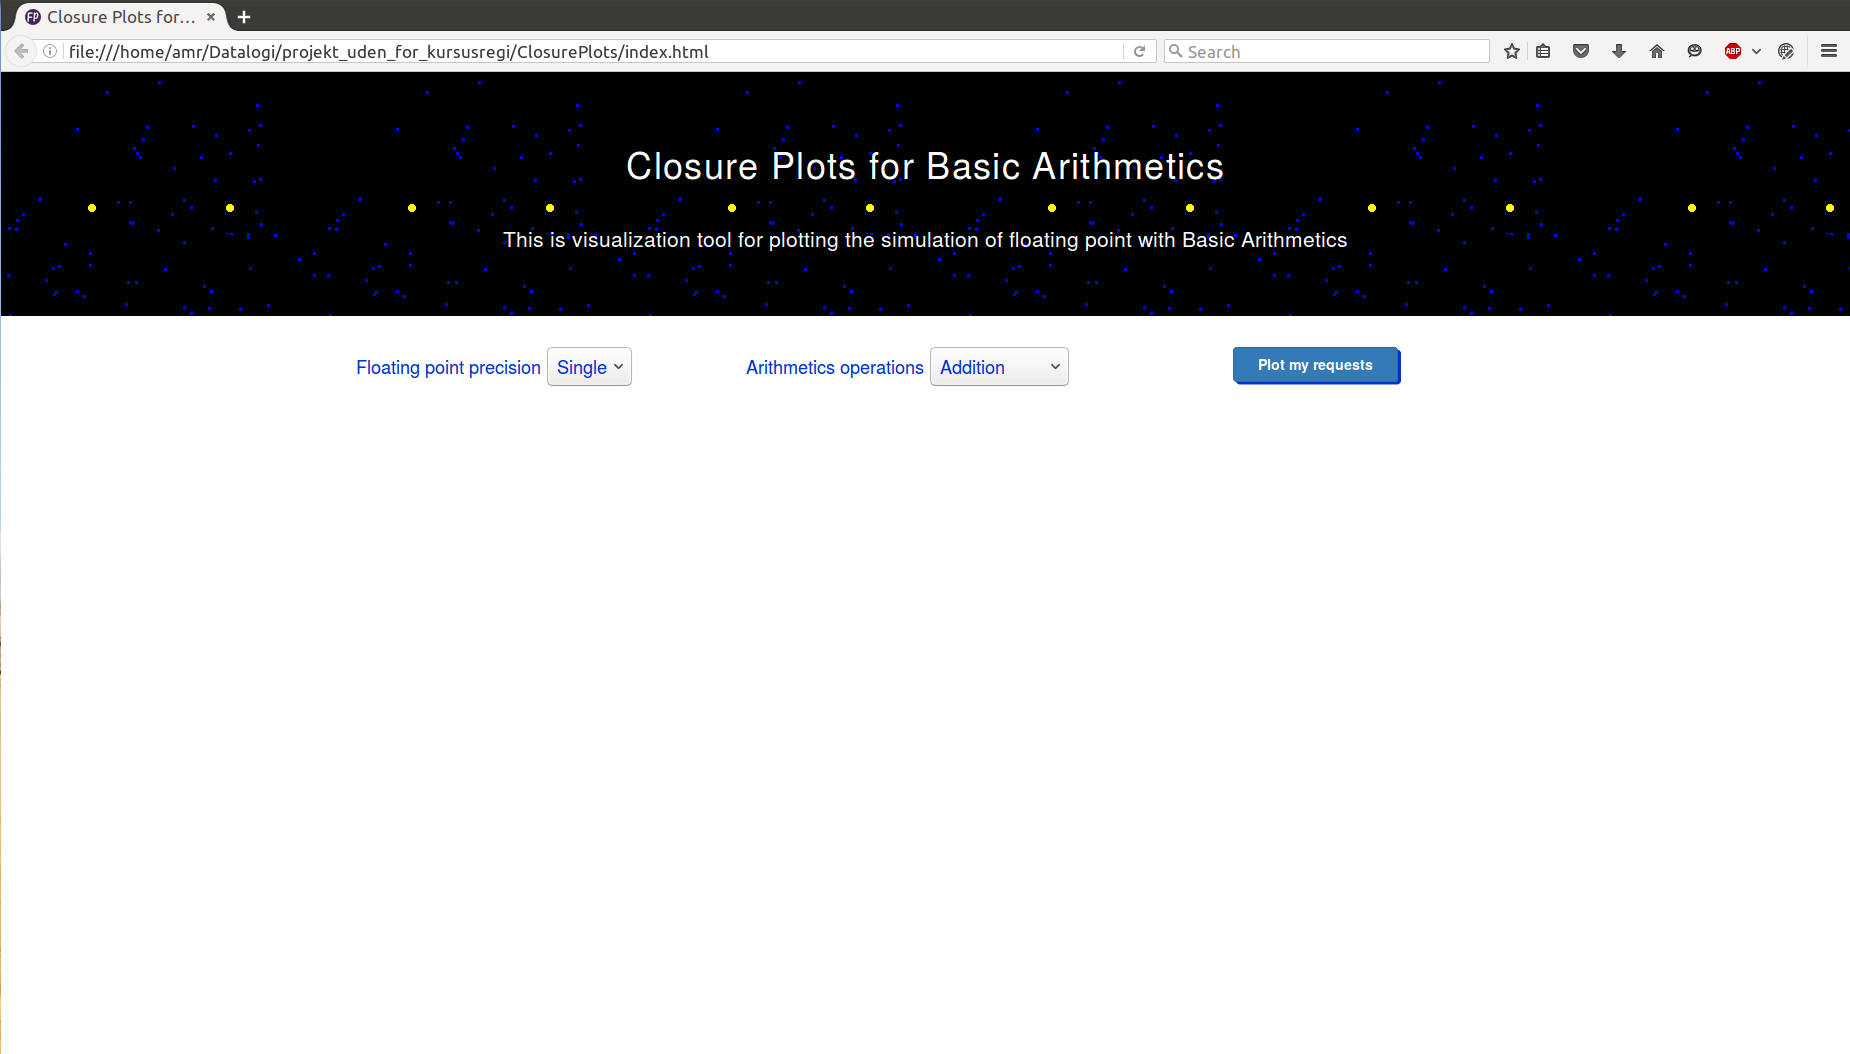
\includegraphics[width=1\textwidth]{layout}
    \caption{CPBA application UI}
    \label{UI}
\end{figure}\\
\subsection{Back-end}
For the implementation of the back-end I have mentioned at design section that i will use javascript to implement the back-end functionality. The back-end are consisting of many functions, I will review these functions based on their order of the implementation to CPBA application.
\subsubsection{getPrecision() function.}
This function is called when the body of webpage has been loaded, and thereafter if the user has change the selec option to precision. getPrecision will get the value of precision select option, which is 16 for Half precision  or 32 for single precision. The function start with initialize the global precArr variable to empty array, and initialize the global mobile variable to 0. Thereafter assign variable temp the return value of base 2 to the exponent power of precision value ( 16 or 32).
Now the function is ready to create the width and height value to the selected precision, and that is done by while loop as long as a specified condition ((temp/16) >= 1) is true. Inside the scope of while loop I divide the value of temp variable by 16 and, and then push the return value of temp -1 to precArr array. The while loop will create array of width and height values.\\

The return value for precArr variable when precision is half will be \textbf{[4095, 255, 15, 0]}, and the return value for precArr when precision is Single will be \textbf{[268435455, 16777215, 1048575, 65535, 4095, 255, 15, 0]}.\\
The JavaScript code for getPrecision() function is show in the code snippet\ref{lst:getPrecision}.\\
\begin{lstlisting}[label={lst:getPrecision}, language=Javascript, caption={getPrecision function},]
/* getPrecision Function is to create array of the different dimensional to chart.
 * The function has to reset mobile variable to zero, which will point to the start of precArr.
 * The function will be execute onload of the body tag and when a user changes the selected option of a <select> element.
 */
var mobile = 0;
var precArr = [];

function getPrecision(){
	precArr = [];
	mobile  = 0;
	var temp= Math.pow(2, document.getElementById("precision").value);

	while((temp / 16) >= 1){
		temp /= 16;
		precArr.push(temp-1); 
	}
}
\end{lstlisting}

\subsubsection{getRequest() function.} 
This function is called when the user has clicked on "Plot my requests" button. The function start with define variable op and assign this variable to the value of select option "operations", which are (addition, subtraction, multiplication, or division). Thereafter define switch statement and evaluate variable "op " value to matching the value to a case clause, and executes function associated with that case.\\
The JavaScript code for getPrecision() function is show in the code snippet\ref{lst:getRequest}.\\
\begin{lstlisting}[label={lst:getRequest}, language=Javascript, caption={getPrecision function},]
/*	getRequest function is to create object of the selected options
 *	and call the appropriate function depending on user request.
 */
function getRequest(){
	var op = document.getElementById("operations").value;
	switch(op){
		case "addition":
			add();
			break;
		case "subtraction":
			sub();
			break;
		case "multiplication":
			mult();
			break;
		case "division":
			divi();
			break;
		default:
			alert('Something went wrong!\n'
				+ 'Please contact the publisher and let the author know about the bug.\n'
				+ 'amr11682@hotmail.com');
			break;
	}
}
\end{lstlisting}

\subsubsection{function add()}
The add() function is to calculate the sum of two variables or more in arithmetic operation , and to show the behaviour of this arithmetic operation ( Correct, overflow ).  It will be executed when it been called from function getRequest().\\
The body of add() function starts with defining variable prec, this variable will be assign to value of precision selected option, thereafter defining variable  range, this variable will be assign to the return value of base 2 to the exponent power of prec value.
The height and width variables are assign to value of precArr[mobile], where precArr and mobile have been created from getPrecision() function.
Thereafter Initialize variable index to 0 and initialize varaible row to empty array. The variable index will be use to insert pecified item to array row. The variables f1 and f2 are defined to assign the values of X and Y to them after convert their values to binary format.\\

The next variable is getPixel, this variable declare function expression in the current scope of add() function. getPixel will summarize 4 edges of 256 element at each stage based on height and width value. In the current scope of getPixel function I defining variable check, this variable declare function expression, this function checking the sum of items at each edge for the 4 edges to 256 elements, if the result of the edge is less than the value of range variable, so increase correct variable by 1,  otherwise increase the variable overflow by 1.\\

The next step is to represent the result of summarized data, and that is done by checking if the value of correct variable is more then 0 and the value of overflow variable is equal to 0, so the summarized data will be shown to user as it is correct data, or if the value of overflow variable is more then 0 and the value of correct variable is equal to 0, so the summarized data will be shown to user as it is overflow data, other than that the summarized data will be shown to user as it is mix data (correct and overflow).\\

At lines 40-42 of the snipped code, I had defined variables xV and yV, those variables will be assigned to the value of variables xValue and yValue. The variables xValue and yValue have been defined as global and have been initialized to null value as shown in the snapped code \ref{lst:xyvalue-global}, therefor at the first stage xV and yV will be assign to 0,  but if the user has clicked on an item of the represented data, so the values of this item will be assign to xValue and yValue variables and thereby xV and yV will be assign to xValue and yValue.\\

The getFormat variable is declare function expression in the current scope of add() function. I had definf getFormat function with one parameter, this parameter will be passing with prec variable to decBin function \ref{lst:decBin}, and the return value of decBin is assign to variables f1 and f2, where those variables will represent the binary value of x and y items of the shown data.\\

At lines 47-57 I had defind two for loop. The first loop will represent the x-axis items, and the second loop will represent the y-axis items.
The first loop has 16 iteration, and in the beginning of the loop I started with assign variable x to the value of variable xV, and at each iteration the x value is updating to its value plus width value. Thereafter I call getFormat function with x value to get the binary value of x, so i can show it to user. The next variable is dicX, this variable is an object with two properties key and value, and it is defined like that to fit Google Chart API for represent the items. The value for v key is x value, and the value of f key is the binary value of f1 to f2.\\
The second loop is defined in the body of the first loop, it has also 16 iteration. I started the same way as the previous loop, but this time with assign variable y to the value of variable yV, and at each iteration the y value is updating to its value plus height value. Thereafter I call getFormat function with y value to get the binary value of y, so i can show it to user. I had defined variable dicY as an object with two properties key and value. The value for v key is y value, and the value of f key is the binary value of f1 to f2. Now I can call getPixel to summarize the 4 edges, and that is done by passing variables x, y , height, width, dicX, and dicY in getPixel function.\\
This two loop produce 256 elements, those elements have been inserted at row array at getPixel function, therefore at line 58 I called drawChart() function for represent the data to user. At the next subsection I will review and explain drawChart() \ref{lst:drawChart} function and how it works.\\
%After a function expression has been stored in a variable, the variable can be used as a function:
\begin{lstlisting}[label={lst:add}, language=Javascript, caption={add function},]
// function to create the simulation of Arithmetics operation ( addition )
function add(){
	var prec  = parseInt(document.getElementById("precision").value);

	var range = Math.pow(2, prec);

	var height= precArr[mobile];
	var width = precArr[mobile];

	var index = 0;
	var rows  = [];

	var f1; // X-axis data format 
	var f2; // Y-axis data format

	var getPixel = function(x, y, height, width, dictX, dictY) {
		var correct = 0;
		var overflow = 0;
		
		var check = function(x,y) {
			if (x + y < range) { correct += 1; } else { overflow += 1; }	
		}
		check(x, y);
		check(x, y + height);
		check(x + width, y);
		check(x + width, y + height);
		if (correct > 0 && overflow == 0) {
	    	// Correct data
			rows[index] = [dictX, dictY, null, null];

		} else if(overflow > 0 && correct == 0) {
			// Overflow data
			rows[index] = [dictX, null, dictY, null];

		} else {
			// Mix data
			rows[index] = [dictX, null, null, dictY];
		}
	}
	var xV;
	var yV; 
	if(xValue == null && yValue == null){xV=0; yV=0;}else{xV = xValue; yV = yValue;}
	if(clickIndex > 0){clickedX.push(xV);clickedY.push(yV);}
	
	var getFormat = function(param){f1 = decBin(param, prec); f2 = decBin(param+height, prec);}
	//var x = 0
	for(var x = xV, i = 0; i < 16; i++, x += width+1){
		getFormat(x);
		var dictX = {v:x, f:'X: '+f1+' to '+f2};
		//var y = 0
		for(var y = yV, j = 0; j < 16; j++, y += height+1){
			getFormat(y);
			var dictY = {v:y, f:'Y: '+f1+' to '+f2};
			getPixel(x, y, height, width, dictX, dictY);
			index += 1;
		}
	}
	drawChart(rows, ['Overflow', 'Mix']);
}
\end{lstlisting}

\begin{lstlisting}[label={lst:xyvalue-global}, language=Javascript, caption={Global variables},]
// Declare global variable, which will get their value from drawChart function, 
// only if the user has interacted with chart ( click on (x,y) ). 
var xValue = null;
var yValue = null;

var clickedX = [];
var clickedY = [];
var clickIndex = 0;
\end{lstlisting}

\begin{lstlisting}[label={lst:decBin}, language=Javascript, caption={Convert (Decimal to Binary) with specify length of the output},]
/*	decBin function is to convert (Decimal to Binary) with specify length of the output.
 *	The function take 2 arguments ( dec, length)
 *	dec   : is the decimal number, which need to be convert to binary
 *	length: is the desirable precision 
 *	The function convert positive decimal as well as negative decimal 
 */
function decBin(dec,length){
	var out = "";
	while(length--)
		out += (dec >> length ) & 1;
	return out;
}
\end{lstlisting}

\subsubsection{function drawChart(arg1, arg2) }

\begin{lstlisting}[label={lst:drawChart}, language=Javascript, caption={drawChart function will visualize the passed data to user.},]
function drawChart(arg1, arg2) {
	// Define the chart to be drawn. 
	var data = new google.visualization.DataTable();
	data.addColumn('number', '');
	data.addColumn('number', 'correct');
	if (arg2.length == 3){
		// numbers do not divide evenly  (Inexpressible) 
		data.addColumn('number', arg2[0]);
		// divide by zero
		data.addColumn('number', arg2[1]);
		// Mixed
		data.addColumn('number', arg2[2]);
	} else{
		// Overflow or Underflow
		data.addColumn('number', arg2[0]);
		// Mixed
		data.addColumn('number', arg2[1]);
	}
   
   	data.addRows(arg1);
    var options = {
    	chart: {
    		title: ' Plotting the simulation of floating point with Basic Arithmetics',
        	//subtitle: 'Based on precision 4 bits'
     	},
     	width: 1150,
     	height: 500,
     	explorer: {
     		actions: ['dragToZoom', 'rightClickToReset'],
        	axis: 'horizontal',
        	keepInBounds: true,
        	maxZoomIn: 4.0
    	},
    };
    var chart = new google.charts.Scatter(document.getElementById('chart_div1'));

    chart.draw(data, google.charts.Scatter.convertOptions(options));
 

	// Listen for the 'select' event, and call my function selectHandler() when
	// the user selects something on the chart.

    google.visualization.events.addListener(chart, 'select', selectHandler);

    // This function to get the index of the selected element of chart.
	function selectHandler() {

		mobile += 1;

		var selectedItemRow = chart.getSelection()[0].row;
		var selectedItemCol = chart.getSelection()[0].column;

		if (selectedItemRow != null){
			//alert(data.getValue(selectedItemRow, 0));
			xValue = data.getValue(selectedItemRow, 0);
			yValue = data.getValue(selectedItemRow, selectedItemCol);

			var valid  = checkIndex();

			if(valid){
				clickIndex += 1;
				//clickedX.push(xValue);
				//clickedY.push(yValue);
				getRequest();//xValue, yValue);
			}
		}
	};
}
\end{lstlisting}
\subsubsection{function sub()}
\begin{lstlisting}[label={lst:sub}, language=Javascript, caption={sub function},]
// function to create the simulation of Arithmetics operation ( subtraction )
function sub(){//xValue, yValue){
	var prec  = parseInt(document.getElementById("precision").value);
	// range to iteration (loop)
	var range = Math.pow(2, prec);

	var height= precArr[mobile];
	var width = precArr[mobile];

	var index = 0;
	var rows  = [];

	var f1; // axis data format 
	var f2; // axis data format

	var getPixel = function(x, y, height, width, dictX, dictY) {
		var correct = 0;
		var underflow = 0;
			// correct logic
			// format is:  x index , correct , overflow
			if ((i-j) >= 0 & (i-j) < range){
				rows[index] = [dictX, dictY, null];
			// else overflow
			}else{
				rows[index] = [dictX, , dictY];
			}


		var check = function(x,y) {
			if ((x - y) >=0 && (x - y) < range) { correct += 1; } else { underflow += 1; }	
		}
		check(x, y);
		check(x, y + height);
		check(x + width, y);
		check(x + width, y + height);
		if (correct > 0 && underflow == 0) {
	    	// Correct data
			rows[index] = [dictX, dictY, null, null];

		} else if(underflow > 0 && correct == 0) {
			// Overflow data
			rows[index] = [dictX, null, dictY, null];

		} else {
			// Mix data
			rows[index] = [dictX, null, null, dictY];
		}
	}
	var xV;
	var yV; 
	if(xValue == null && yValue == null){xV=0; yV=0;}else{xV = xValue; yV = yValue;}
	if(clickIndex > 0){clickedX.push(xV);clickedY.push(yV);}
	
	var getFormat = function(param){f1 = decBin(param, prec); f2 = decBin(param+height, prec);}
	//var x = 0
	for(var x = xV, i = 0; i < 16; i++, x += width+1){
		getFormat(x);
		var dictX = {v:x, f:'X: '+f1+' to '+f2};
		//var y = 0
		for(var y = yV, j = 0; j < 16; j++, y += height+1){
			getFormat(y);
			var dictY = {v:y, f:'Y: '+f1+' to '+f2};
			getPixel(x, y, height, width, dictX, dictY);
			index += 1;
		}
	}
	drawChart(rows, ['Underflow', 'Mix']);
}
\end{lstlisting}

\subsubsection{function mult()}
\begin{lstlisting}[label={lst:mult}, language=Javascript, caption={mult function},]
// function to create the simulation of Arithmetics operation ( multiplication )
function mult(){//xValue, yValue){
	var prec  = parseInt(document.getElementById("precision").value);
	// range to iteration (loop)
	var range = Math.pow(2, prec);

	var height= precArr[mobile];
	var width = precArr[mobile];

	var index = 0;
	var rows  = [];

	var f1; // axis data format 
	var f2; // axis data format

	var getPixel = function(x, y, height, width, dictX, dictY) {
		var correct = 0;
		var overflow = 0;

		var check = function(x,y) {
			if (x * y < range) { correct += 1; } else { overflow += 1; }	
		}
		check(x, y);
		check(x, y + height);
		check(x + width, y);
		check(x + width, y + height);
		if (correct > 0 && overflow == 0) {
	    	// Correct data
			rows[index] = [dictX, dictY, null, null];

		} else if(overflow > 0 && correct == 0) {
			// Overflow data
			rows[index] = [dictX, null, dictY, null];

		} else {
			// Mix data
			rows[index] = [dictX, null, null, dictY];
		}
	}
	var xV;
	var yV; 
	if(xValue == null && yValue == null){xV=0; yV=0;}else{xV = xValue; yV = yValue;}
	if(clickIndex > 0){clickedX.push(xV);clickedY.push(yV);}
	
	var getFormat = function(param){f1 = decBin(param, prec); f2 = decBin(param+height, prec);}
	
	for(var x = xV, i = 0; i < 16; i++, x += width+1){
		getFormat(x);
		var dictX = {v:x, f:'X: '+f1+' to '+f2};
		//var y = 0
		for(var y = yV, j = 0; j < 16; j++, y += height+1){
			getFormat(y);
			var dictY = {v:y, f:'Y: '+f1+' to '+f2};
			getPixel(x, y, height, width, dictX, dictY);
			index += 1;
		}
	}
	drawChart(rows, ['Overflow', 'Mix']);
}

\end{lstlisting}

\subsubsection{function divi()}
\begin{lstlisting}[label={lst:divi}, language=Javascript, caption={divi function},]
// function to create the simulation of Arithmetics operation ( division )
function divi(){//xValue, yValue){
	var prec  = parseInt(document.getElementById("precision").value);
	// range to iteration (loop)
	var range = Math.pow(2, prec);

	var height= precArr[mobile];
	var width = precArr[mobile];

	var index = 0;
	var rows  = [];

	var f1; // axis data format 
	var f2; // axis data format

	var getPixel = function(x, y, height, width, dictX, dictY) {
		var correct = 0;
		var infi    = 0;
		var Inexpressible = 0;

		var check = function(x,y) {
			if ((x/y) % 1 == 0) { correct += 1; }
			else if(isNaN(x/y) || !(isFinite(x/y))) { infi += 1;}
			else{ Inexpressible += 1; }	
		}
		check(x, y);
		check(x, y + height);
		check(x + width, y);
		check(x + width, y + height);
		if (correct > 0 && Inexpressible == 0 && infi == 0) {
	    	// Correct data: does (1/3) which is 0.33.. mod 1  equal to zero
			rows[index] = [dictX, dictY, null, null, null];

		} else if(Inexpressible > 0 && correct == 0 && infi == 0) {
			// Inexpressible data
			rows[index] = [dictX, null, dictY, null, null];

		}else if(infi > 0 && correct == 0 && Inexpressible == 0) {
			// check if is NAN eg. 0/0  or is Infinity(not finite)  eg. 1/0 , 1000/0
			rows[index] = [dictX, null, null, dictY, null];

		} else {
			// Mix data
			rows[index] = [dictX, null, null, null, dictY];
		}
	}
	var xV;
	var yV; 
	if(xValue == null && yValue == null){xV=0; yV=0;}else{xV = xValue; yV = yValue;}
	if(clickIndex > 0){clickedX.push(xV);clickedY.push(yV);}
	
	var getFormat = function(param){f1 = decBin(param, prec); f2 = decBin(param+height, prec);}
	
	for(var x = xV, i = 0; i < 16; i++, x += width+1){
		getFormat(x);
		var dictX = {v:x, f:'X: '+f1+' to '+f2};
	
		for(var y = yV, j = 0; j < 16; j++, y += height+1){
			getFormat(y);
			var dictY = {v:y, f:'Y: '+f1+' to '+f2};
			getPixel(x, y, height, width, dictX, dictY);
			index += 1;
		}
	}
	drawChart(rows, ['Inexpressible', 'infinity','Mix']);
}
\end{lstlisting}
\section{Testing}
%\section{Future Development}

%\section{Work progress}


\section{Conclusion}

\section*{Footnotes}
\begin{itemize}
\item \url{http://steve.hollasch.net/cgindex/coding/ieeefloat.html}
\end{itemize}
\addcontentsline{toc}{section}{appendices}
\appendix
\begin{appendices}

\end{appendices}

\end{document}
